\documentclass{article}%
\usepackage{amsmath}%
\usepackage{amsfonts}%
\usepackage{amssymb}%
\usepackage{graphicx}
%-------------------------------------------
\newtheorem{theorem}{Theorem}
\newtheorem{acknowledgement}[theorem]{Acknowledgement}
\newtheorem{algorithm}[theorem]{Algorithm}
\newtheorem{axiom}[theorem]{Axiom}
\newtheorem{case}[theorem]{Case}
\newtheorem{claim}[theorem]{Claim}
\newtheorem{conclusion}[theorem]{Conclusion}
\newtheorem{condition}[theorem]{Condition}
\newtheorem{conjecture}[theorem]{Conjecture}
\newtheorem{corollary}[theorem]{Corollary}
\newtheorem{criterion}[theorem]{Criterion}
\newtheorem{definition}[theorem]{Definition}
\newtheorem{example}[theorem]{Example}
\newtheorem{exercise}[theorem]{Exercise}
\newtheorem{lemma}[theorem]{Lemma}
\newtheorem{notation}[theorem]{Notation}
\newtheorem{problem}[theorem]{Problem}
\newtheorem{proposition}[theorem]{Proposition}
\newtheorem{remark}[theorem]{Remark}
\newtheorem{solution}[theorem]{Solution}
\newtheorem{summary}[theorem]{Summary}
\newenvironment{proof}[1][Proof]{\textbf{#1.} }{\ \rule{0.5em}{0.5em}}
\setlength{\textwidth}{7.0in}
\setlength{\oddsidemargin}{-0.35in}
\setlength{\topmargin}{-0.5in}
\setlength{\textheight}{9.0in}
\setlength{\parindent}{0.3in}
\begin{document}

\begin{flushright}
\textbf{Ziad Arafat \\
FEB 10, 2017}
\end{flushright}

\begin{center}
\textbf{MATH190G: Trigonometry and Precalculus \\
Exam I Corrections} \\
\end{center}
\section*{1.}
\textbf{Determine if the point $(\frac{-5\sqrt[]{3}}{9}, \frac{-1}{\sqrt[]{6}})$ is on the unit circle.}
\begin{center}
It does not lie on the unit circle.
A point with coordinates $(a,b)$ is on the unit circle if and only if: \newline
$a^2 + b^2 = 1$

The unit circle by defintion is a circle with radius 1 with center $(0,0)$, so the distance of the points $(x,y)$ in that circle to the center is equal to 1. So by the distance formula: \newline
$\sqrt[]{a^2+b^2} = 1 \iff a^2+b^2=1$

$(-5 \sqrt[]{3}/9)^2 + (-1/\sqrt[]{6})^2 = 1.92...$ \newline
$(-5 \frac{\sqrt[]{3}}{9})^2 + (\frac{-1}{\sqrt[]{6}})^2 \neq 1$
\end{center}
\section*{2. through 13.}
\begin{small}
(all correct)
\end{small}

\section*{14.}
\textbf{Given the terminal point $P(-5, 12)$ of a real number $t$, find the exact value for: }

(calculator syntax mistake)
\begin{center}
$(-15)^2 + (12)^2 = 169$ \newline
$\sqrt[]{169} = 13$ \newline

$sin(t) = \frac{12}{13}$, $cos(t) = \frac{-5}{13}$, $tan(t) = \frac{-12}{5}$, $csc(t) = \frac{13}{12}$, $sec(t) = -\frac{13}{5}$, $sin(t) = \frac{-5}{12}$ 

\end{center}

\section*{15. through 19.}
\begin{small}
(all correct)
\end{small}

\section*{20.}


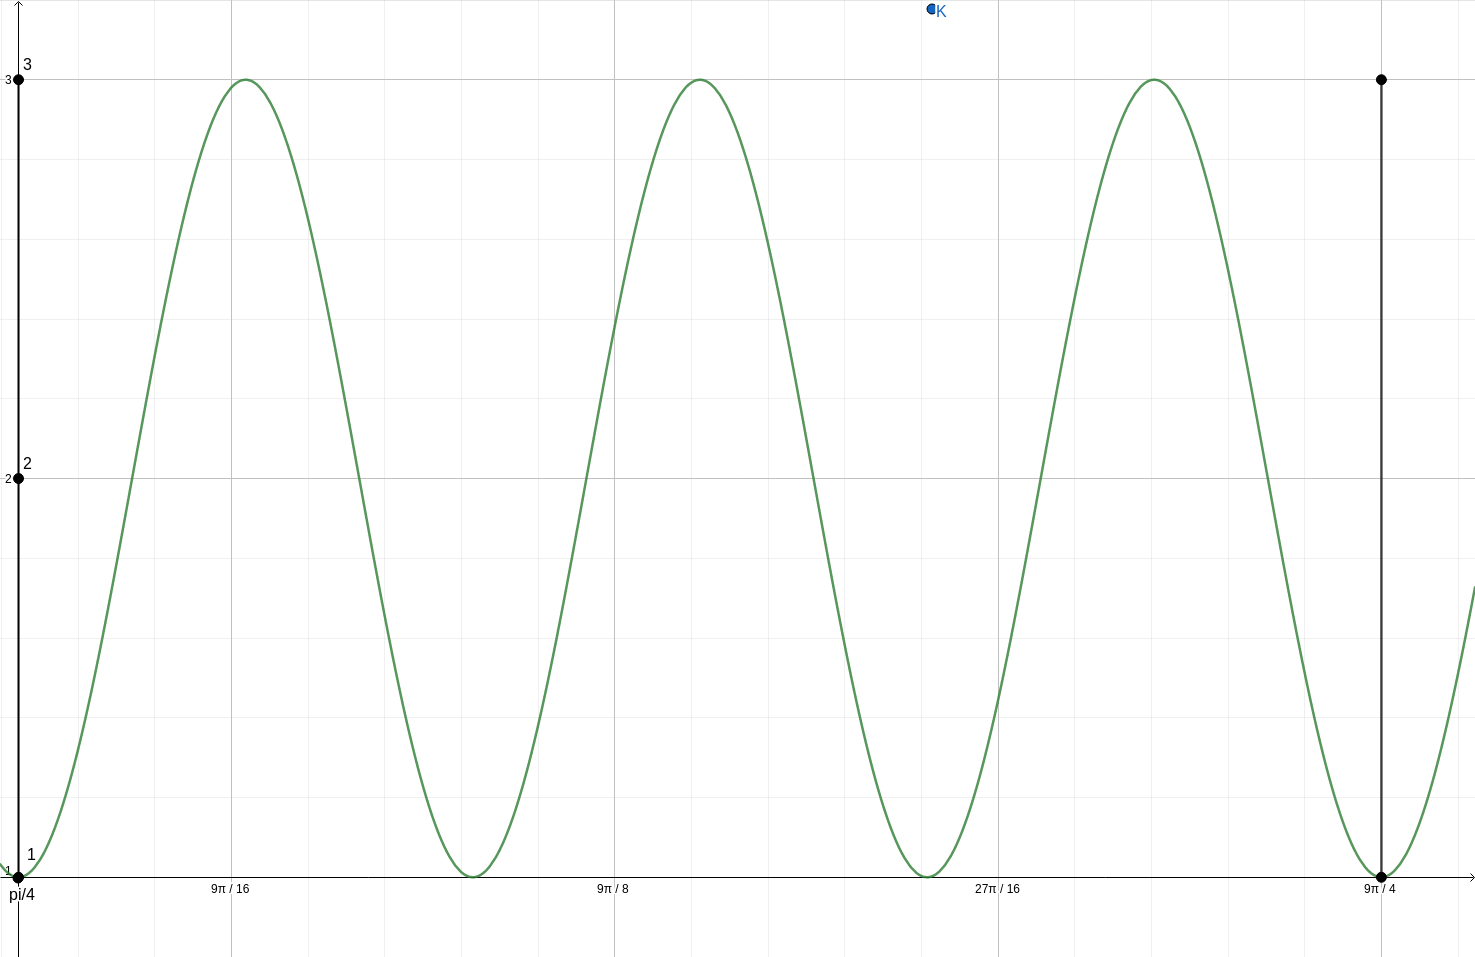
\includegraphics[scale=0.4]{/home/cat/Documents/notes/MATH190G/Exam1.png}
\section*{21. and 22.}
\begin{small}
(all correct)
\end{small}
\clearpage
\section*{23.}
\textbf{Write a cosine function that models the simple harmonic motion having the given properties. Assume that the displacement is at its maximum at time $t = 0$. The amplitude is $4.25$ meters and the wave has a frequency of $256$ Hz. \newline}

\begin{center}
$f(x) = +4.25\cos (512\pi t)$\newline

$P=\frac{2\pi}{b}$\newline
$256\times 2 = 512 = \frac{2\pi}{b}$\newline
\end{center}



\section*{24.}
\textbf{A certain cove with very high tides displays the following behavior. In one $12$-hour period, the water starts at the mean sea level, rises $23$ feet before reaching its maximum tidal height before receding to its minimum height, and then returns to mean sea level. Assuming that the motion of the tide is simple harmonic in nature, write a sine function that can be used to predict the height of the tide at any given time. \newline}
\begin{center}
$y = 23\sin(\frac{\pi}{6}(t))$ \newline \newline
$\frac{2pi}{b} = 12$\newline
$2\pi = 12b$\newline
$b = \frac{2\pi}{12}$\newline
$b = \frac{\pi}{6}$\newline
\end{center}

\section*{25.}
\textbf{Use the given information to write a sine function that models the relationship between time and the barn owl population in a particular town. }

\subsection*{25.1}
\textbf{Show your work as to how you determined the amplitude. \newline}

\begin{center}
$Max-Min=80-20=60$\newline
$60\div 2 = 30$\newline
$amp=30$\newline
\end{center}
\subsection*{25.2}
\textbf{Show your work as to how you determined the equilibrium point. \newline}
\begin{center}
$Min+amp = 20+30 = 50$ \newline
$equilibrium=50$\newline
\end{center}


\subsection*{25.3}
\textbf{Describe how you determined the period of the function. \newline}
Equilibrium occurs at $t=6$ and $t=12$. $12-6=6$, So the frequency is $6$. $period = 2\times frequency = 2\times 6= 12$
$period=12$
$\frac{2\pi}{12} = \frac{\pi}{6}$
\subsection*{25.4}
\textbf{Describe how you determined the phase shift of the function. \newline}
Since we start at $t=1$ and equillibrium starts at $t=6$ the phase shift is $6$ units right.
$x-6$
\subsection*{25.5}
\textbf{Answer: }
$T = 50-30sin(\frac{\pi}{6}(t-6))$

\vspace*{0.5in}
\noindent Done in LaTeX
\end{document}
